\begin{frame}[allowframebreaks]{}
    \centering
    \LARGE Key Components and Architectures
\end{frame}

\begin{frame}[allowframebreaks]{Key Components and Architectures}
    \begin{itemize}
        \item Imagine you want to predict the next value in a sequence, like the next note in a song or the next pixel in an image.
        \item Autoregressive models help us do this by looking at what has come before.
        \item They learn patterns by using previous values to guess what comes next.
        \item These models are widely used for things like time series forecasting and generating new data.
    \end{itemize}

    \begin{figure}
    \centering
    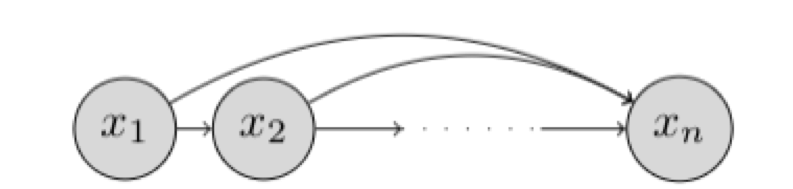
\includegraphics[height=0.5\textheight, width=\textwidth, keepaspectratio]{images/autoregressive/autoregressive.png}
    \caption*{Graphical model for an autoregressive network}
\end{figure}

\framebreak

\begin{itemize}
    \item In the MNIST dataset example, we can set an ordering for all the random variables from top-left $X_1$ to bottom-right $X_{784}$
    \item Without loss of generality, we can use chain rule for factorization
    $$\mathcal{P}(x_1, \cdots, x_{784}) = \mathcal{P}(x_1) \mathcal{P}(x_2|x_1) \mathcal{P}(x_3|x_1, x_2) \cdots \mathcal{P}(x_{784}|x_1, x_2, \cdots, x_{784})$$
    \item Parameterizing the above and using the sigmoid function for binarization,
    \begin{itemize}
        \item $\mathcal{P}_{CPT}(X_1=1;\alpha^1) = \alpha^1, \mathcal{P}(X_1=0) = 1-\alpha^1$
        \item $\mathcal{P}_{logit}(X_2=1|x_1;\alpha^2) = \sigma (\alpha_0^2 + \alpha_1^2 x_1)$
        \item $\mathcal{P}_{logit}(X_3=1|x_1,x_2;\alpha^3) = \sigma (\alpha_0^3 + \alpha_1^3 x_1 + \alpha_2^3 x_2)$
    \end{itemize}
\end{itemize}
\end{frame}